\begin{tikzpicture}[scale=0.9]
\draw[->, thick] (0,0) -- (6.4,0) node[right] {$\sigma$};
\draw[<->, thick] (0,-1.4) -- (0,3) node[above] {$h(X)$ nats};
% h = 0.5 ln(2 pi e s^2) = ln(s) + 1.419 ; zero at s ~ 0.242
% scale: x = s*2.4 (s 0..2.5), y = (ln s + 1.419)*1.3
\draw[very thick, domain=0.24:6.2, smooth, samples=80]
  plot (\x, {1.3*(ln(\x/2.4) + 1.419)});
\fill ({2.4*0.242},0) circle (1.4pt) node[below right] {$\sigma\approx0.24$: $h=0$};
\foreach \x/\xl in {2.4/1, 4.8/2}
  \draw (\x,0.06) -- (\x,-0.06) node[below] {\xl};
\draw[gray, dashed] (0,0) -- (6.2,0);
\node[align=left, anchor=west] at (3.4,-1.0) {$h=\tfrac12\ln(2\pi e\sigma^2)$\\
  differential entropy can be\\ negative --- it is not\\ information, just spread.};
\end{tikzpicture}
